%% -*- mode: latex; mode: flyspell -*-
\documentclass[12pt, letter]{article}

%% Class name and Assignment number
%%
\newcommand{\courseName}{CSC421: Artificial Intelligence}
\newcommand{\assignName}{Assignment~4}

%% Packages
\usepackage{amsmath,amsfonts,amssymb,amsthm,dsfont}
\usepackage{physics}
\usepackage{graphicx}
\usepackage[bookmarks=false]{hyperref}
\usepackage{color}
\usepackage{lipsum}
\usepackage{placeins}
\usepackage{float}
\restylefloat{table}

%% Paper format
\usepackage{geometry}
\geometry{
    letterpaper,
    %% total={216mm,279mm}, %< NSERC size
    margin=2.00cm,     %< default
    %% margin=1.87cm,       %< NSERC tightest
}

%% Headers and footers
\usepackage[explicit]{titlesec}
\newpagestyle{titlesec_assignment}{
  \sethead{\courseName}{}{\assignName}\setfoot{}{\thepage}{}
  \headrule
  %% \footrule
}

\begin{document}

%% Set header and footer
\pagestyle{titlesec_assignment}

%% Title
\title{\courseName\\\assignName}
\author{Rafael Solorzano}
\maketitle

\section{Introduction}

In this assignment logic programming using logpy as well as a standard python is performed for a family tree logic. Further. Hidden Markov Models in python using hmmlearn is performed, to examine different states of healthy or unhealthy as well as moves performed according to this hidden states. 

\section{Logic Programming}

\subsection{logpy}

Logic programming to determine parents, grandparents and children of different Star Wars characters was performed using logpy. First, the parent relationship is created as facts in which we state ("Parent", "Children") the relationships created for this problem is shown in Figure 1. Once the relationships have been created we can query direct results from them, we query "Who is the parent of Luke Skywalker" as well as "Who are the children of Darth Vader" the code for this queries is shown in Figure 2. Finally, in order to query "Who is the grandparent of Kylo Ren?" we first create a an auxiliary grandparent function, and then we query using this new function, the code for this is shown in Figure 3. The results of all these functions is shown in Figure 4.

 \begin{figure}[htb]
  \centering
  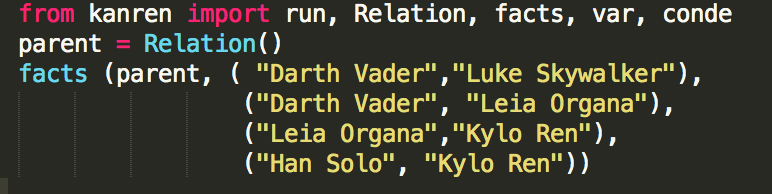
\includegraphics[width=0.75 \textwidth]{./figures/facts_logpy.png}
  \caption{Facts created for the parent relationship using logpy..}
\end{figure}

 \begin{figure}[htb]
  \centering
  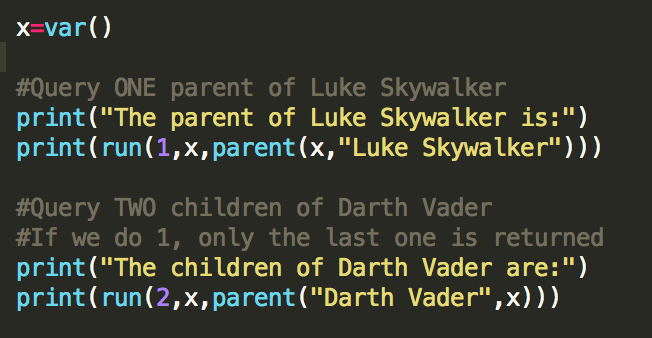
\includegraphics[width=0.70 \textwidth]{./figures/query_ld.png}
  \caption{Query for parent of Luke and children of Darth Vader.}
\end{figure}

 \begin{figure}[htb]
  \centering
  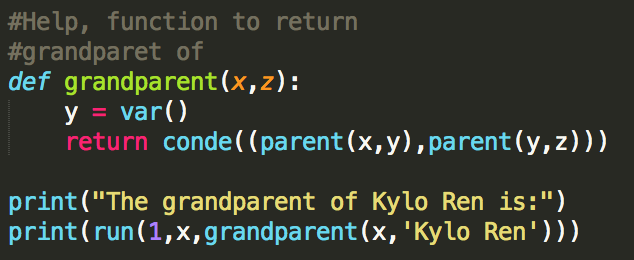
\includegraphics[width=0.65 \textwidth]{./figures/kylo.png}
  \caption{Grandparent function, and query for grandparent of Kylo Ren.}
\end{figure}

 \begin{figure}[htb]
  \centering
  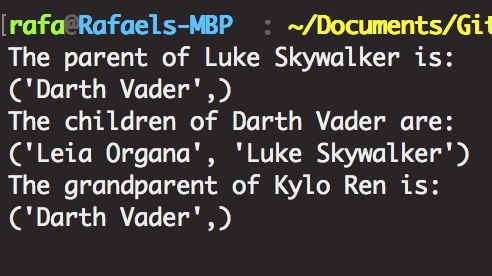
\includegraphics[width=0.50 \textwidth]{./figures/result_log.png}
  \caption{Result of all queries performed in Figures 2 and 3.}
\end{figure}

\FloatBarrier

\subsection{Standard Python}

The same problem with the same queries is also performed using Standard Python. We use a dictionary of lists to establish the facts, this is created in the form "Parent" : ["Child 1" ... "Child n"]. Storing the facts this way, allows us to query for direct children, as well as using a function we can query for every parent of a child, by checking if a child is listed under a parent. Finally, in order to perform the grandparent check, we get the parents of the grandson first, further we get the parents of the parents of the grandson, in the same manner as in parent function. The entire code using Standard Python is shown in Figure 6, and its result is shown in Figure 5. 

 \begin{figure}[htb]
  \centering
  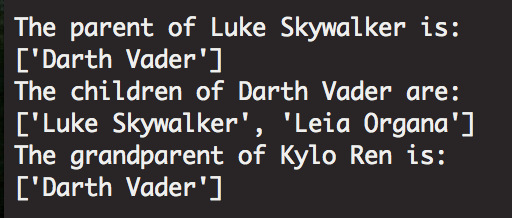
\includegraphics[width=0.55 \textwidth]{./figures/standard_result.png}
  \caption{Results from the Standard Python Implementation.}
\end{figure}

Contrasting the two methods, the logic programming allows for easier and faster queries as well as more robust results. Using logpy or Prolog allow for easy and robust logic programming, with very strong query processing. Whereas, with standard python using dictionaries we have to define every single function of what we want to achieve, and provide precise results of how to do this.  For this particular problem as it is very small set, doing it wit logpy yielded with a lot less code, and only one extra function being needed, whereas for standard Python we required a separate function for each problem that we later can call to get the results. 

 \begin{figure}[htb]
  \centering
  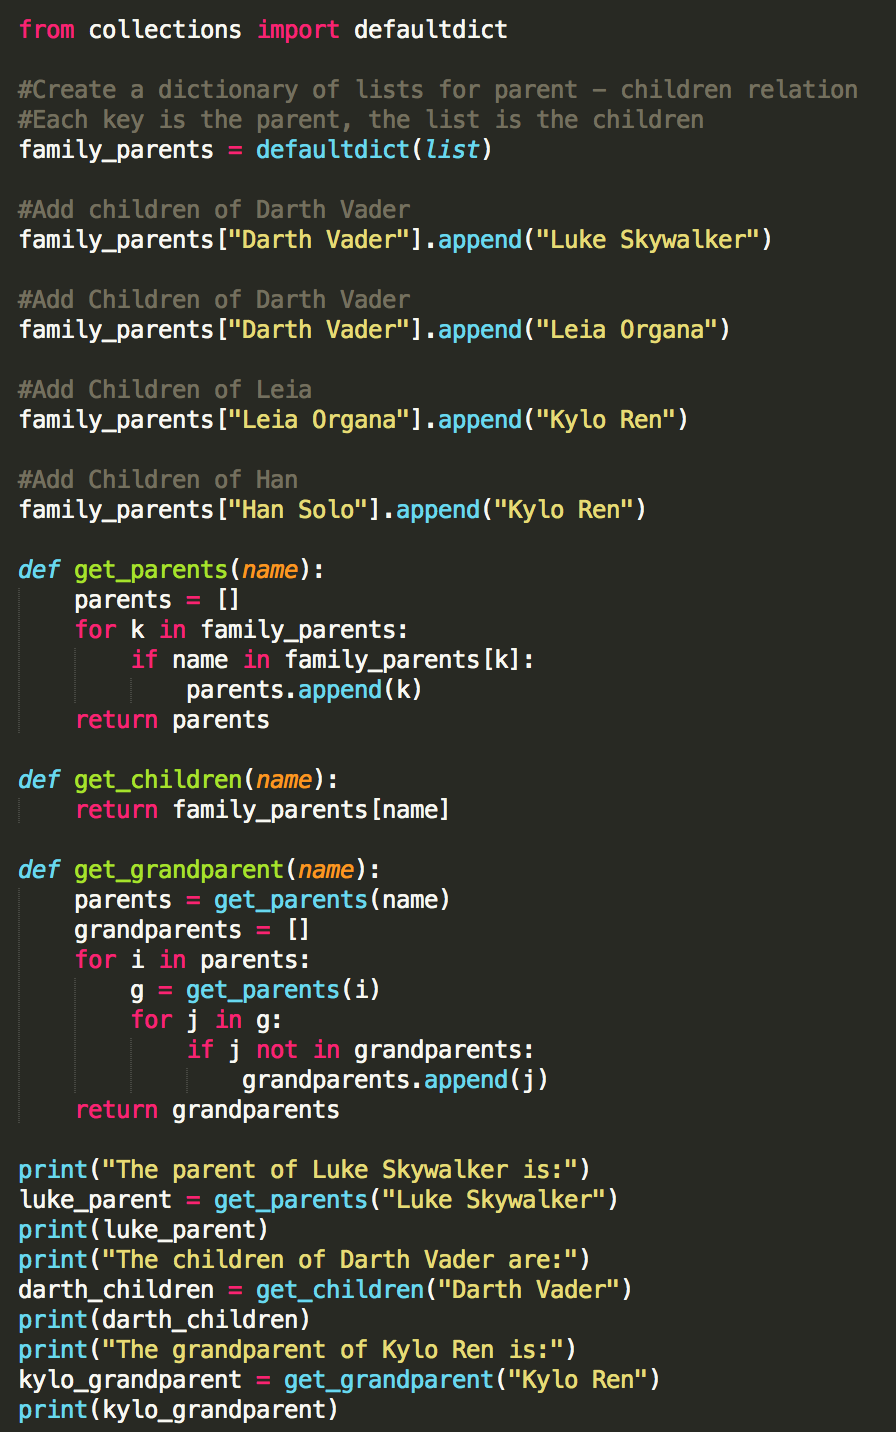
\includegraphics[width=0.80 \textwidth]{./figures/standard_py.png}
  \caption{Standard Python implementation of section 2.1.}
\end{figure}

\FloatBarrier


\section{Hidden Markov Models}

In order to generate random sequence of healthy, and injured an approach similar to the card deck in Monopoly is used. A list of different states labeled 1 for Healthy and 0 for injured is created. For example the healthy matrix would contain 7 1's and 3 0's to represent 0.7 probability of staying healthy and 0.3 of going injured. Further, to generate random sequences of dribble, pass, or shoot given the current state is doing in the same manner as for healthy injured with the difference that 2 represents dribble, 3 represents pass, and 4 represents shoot. The code for the generation of health and injured sequence  is shown in Figure 7, whereas the code for the generation of moves sequence is shown in Figure 8. Finally, a sample printout of each function is shown in Figure 9. 

 \begin{figure}[htb]
  \centering
  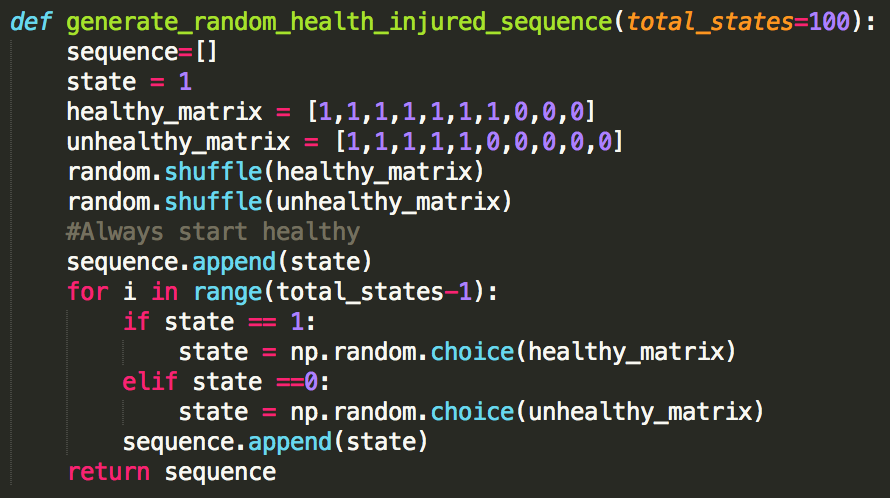
\includegraphics[width=0.70 \textwidth]{./figures/h_i_seq.png}
  \caption{Sequence of random Healthy and Injured generation.}
\end{figure}

 \begin{figure}[htb]
  \centering
  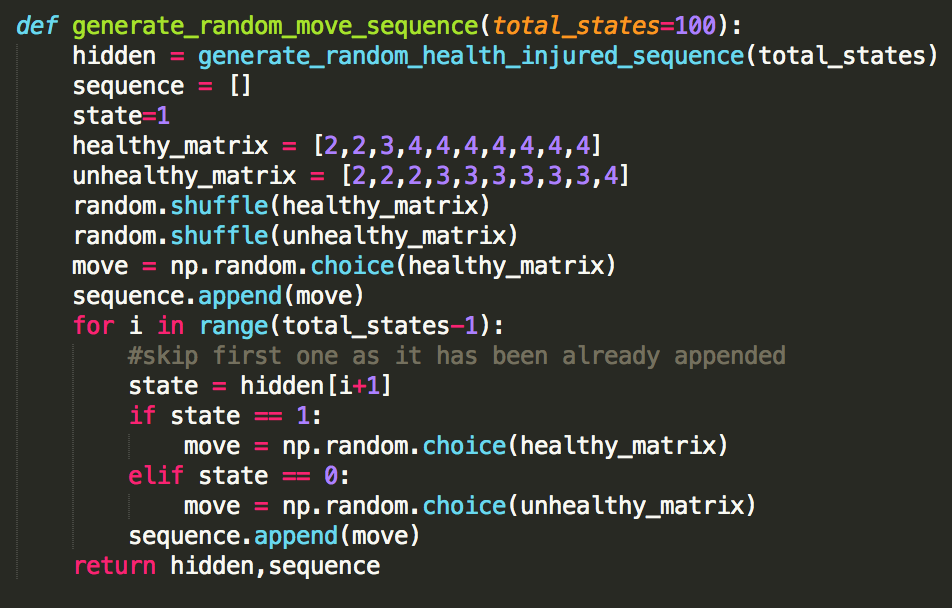
\includegraphics[width=0.70 \textwidth]{./figures/move_seq.png}
  \caption{Sequence of random moves sequence generation.}
\end{figure}

 \begin{figure}[htb]
  \centering
  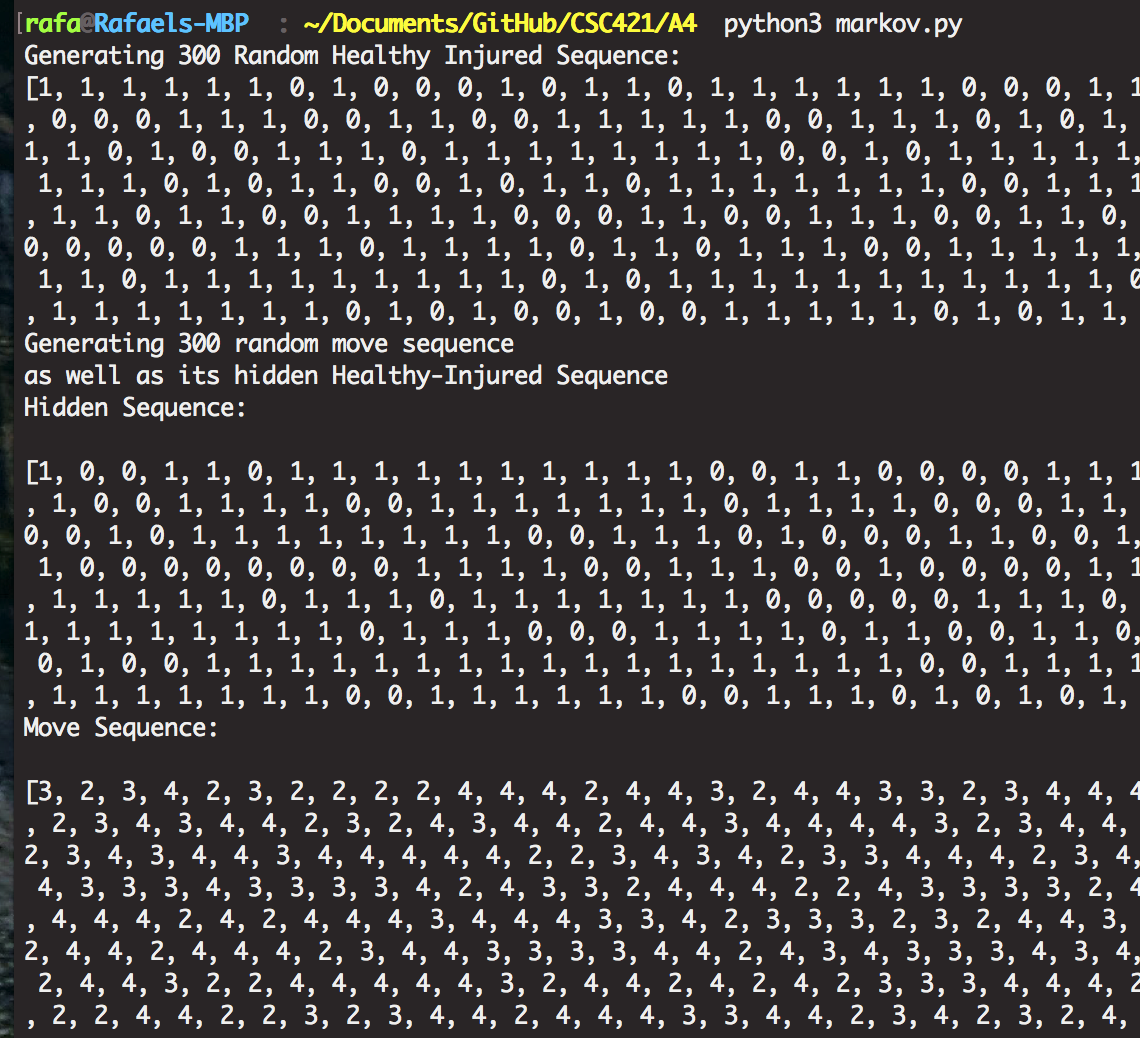
\includegraphics[width=0.80 \textwidth]{./figures/sequence_example.png}
  \caption{A sample sequence generation result.}
\end{figure}

\FloatBarrier

After we have created the sequence of observations, we create a Hidden Markov Model using hmmlearn with Multinomial Hidden Markov Model. First, we create the model object to which we assign the initial probabilities, this are 1.0 and 0.0 as the initial state is always healthy not chosen by random. Second, we define the transition matrix from this states. Third, the emission probability of the different moves is specified. The code for the creation of this model is shown in Figure 10.

 \begin{figure}[htb]
  \centering
  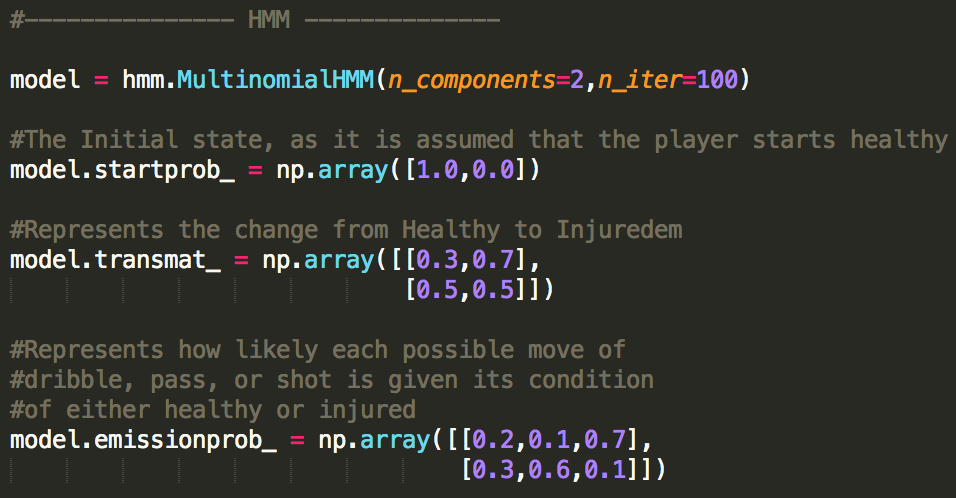
\includegraphics[width=0.70 \textwidth]{./figures/hmm_creation.png}
  \caption{Creation of the Multinomial HMM model.}
\end{figure}

\FloatBarrier

Once we have the model we can fit the generated sequence of moves into our model. After fitting we can sample the model to generate a random sample from it. The code of fit and the printout of the sample results is shown in Figure 11 and 12 respectively.

 \begin{figure}[htb]
  \centering
  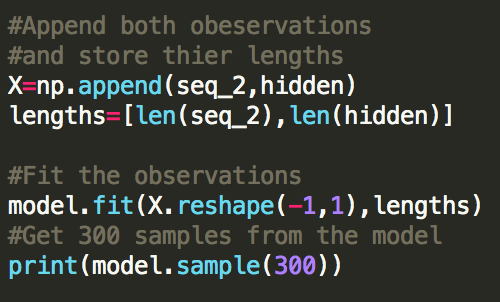
\includegraphics[width=0.50 \textwidth]{./figures/fit.png}
  \caption{Code to fit the sequences into the model.}
\end{figure}

 \begin{figure}[htb]
  \centering
  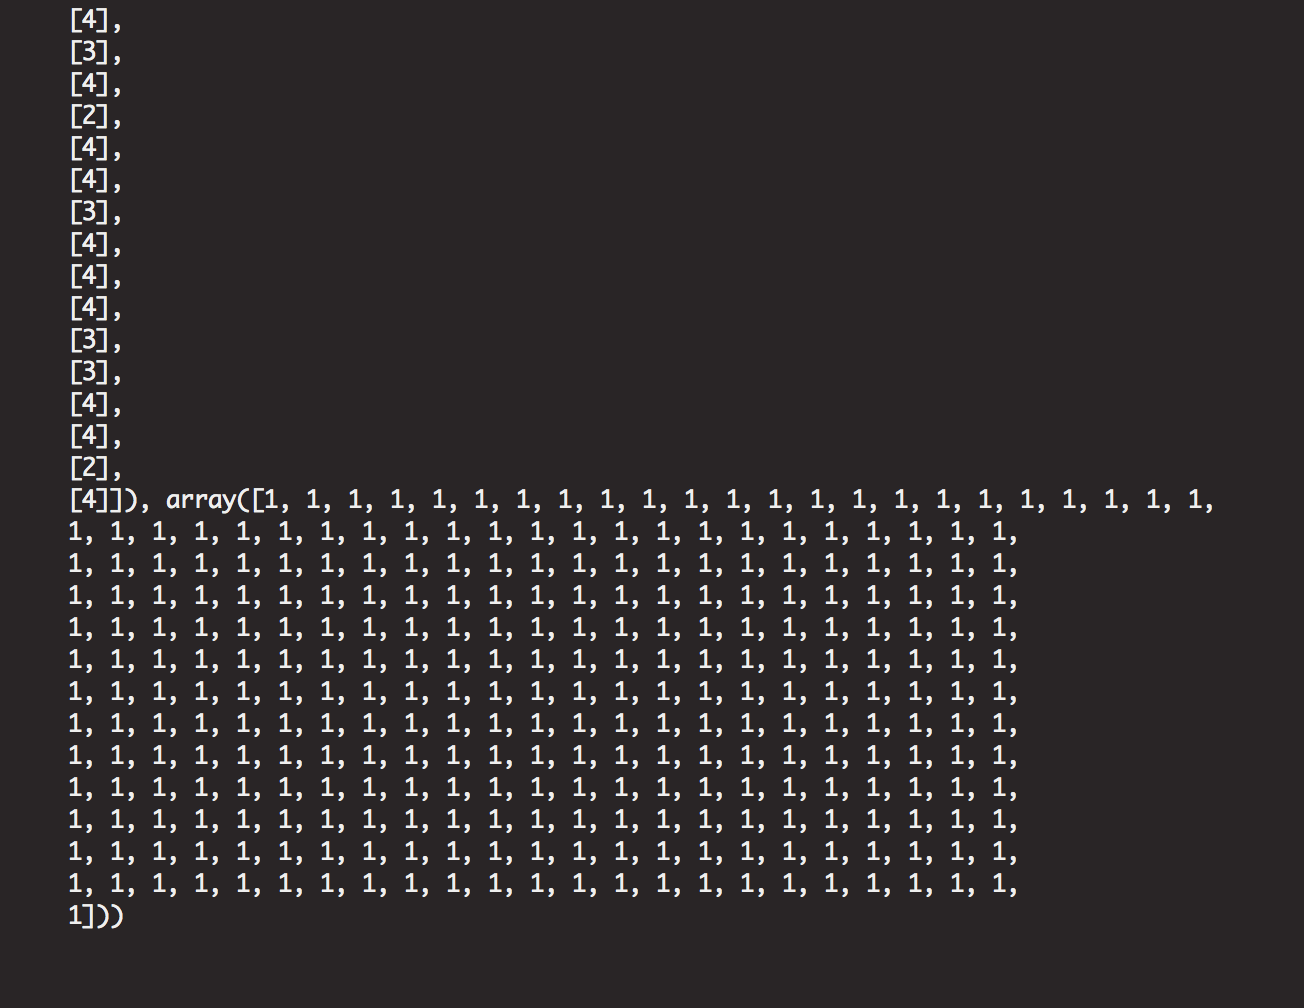
\includegraphics[width=0.80 \textwidth]{./figures/samples.png}
  \caption{The random generation of samples from the code in Figure 11.}
\end{figure}

\FloatBarrier

The predict function of the HMM model will predict the sequence of hidden states, that was used to generate our sequence of observations. It was decided to run this predict function 10 times with different observations and report the results in order to provide how many errors the predict function produced in different runs. The code that does the predict is shown in Figure 13. The error results obtained for each run were:

\begin{itemize}
\item 97
\item 108
\item 173
\item 194
\item 120
\item 107
\item 177
\item 111
\item 202
\item 117
\end{itemize}

 \begin{figure}[htb]
  \centering
  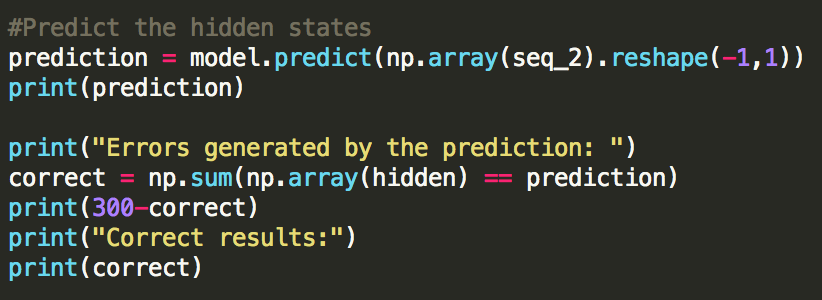
\includegraphics[width=0.70 \textwidth]{./figures/predict.png}
  \caption{The predict function.}
\end{figure}


\end{document}



%%% Local Variables:
%%% mode: latex
%%% TeX-master: t
%%% End:
